

%%%%%%%%%%%%%%%%%%%%%% 
%%%%%%%%%%%%%%%%%%%%%% section 105
%%%%%%%%%%%%%%%%%%%%%% 


\section[Aplicaciones]{Aplicaciones de Ecuaciones Diferenciales de Primer Orden}

\subsection{Crecimiento y decaimiento}


	Sea $N(t)$ la cantidad de algún recurso, sustancia o población que (de-)crece respecto del tiempo.
	
	En este caso $N'(t)$ la tasa de cambio y supondremos que es proporcional a $N(t):$
	
	\[
		\label{bron:7.1}
		\dfrac{dN}{dt}=rN,
	\]
	donde $r$ es la constante de proporcionalidad.



	\begin{problema}
		Una persona deposita $\$20,000$ en una cuenta de ahorros que paga el 5\% de interés  anual, compuesto continuamente.
		Encuentre
		\begin{enumerate}
			\item el monto en la cuenta después de tres años;  
			\item el tiempo requerido para que la cuenta al doble de su valor, sin contar retiros ni depósitos extras.
		\end{enumerate}
		
	\end{problema}
	


\subsection{Ejemplos de enfriamiento}


	La ley de enfriamiento de Newton establece que \emph{la tasa de cambio de la temperatura de un cuerpo (respecto del tiempo) es proporcional a la diferencia entre el cuerpo y el medio circundante:}
	
	\[
		\label{bron:7.2}
		\dfrac{dT}{dt}=-k\left( T-T_{m} \right)
	\]
	donde $k$ es una constante (positiva) de proporcionalidad; $T$ es la temperatura del cuerpo; y $T_{m}$ es la temperatura del medio.


% 
%  \begin{problema}
%   Una barra de metal a una temperatura de $100^\circ F$ es ubicado en un cuarto a una temperatura constante de $0^\circ F.$ Si después de 20 minutos, la temperatura de la barra es de $50^\circ F,$ encuentre:
%   \begin{enumerate}
%    \item el tiempo que tomará alcanzar $25^\circ F$ y;
%    \item la temperatura de la barra después de 10 minutos.
%   \end{enumerate}
%
%  \end{problema}
%
% 
{}
	\begin{problema}
		Un cuerpo a una temperatura de $50^{o}F$ está colocado en el exterior donde la temperatura es de $100^{o}F.$ Si después de 5 minutos la temperatura del cuerpo es $60^{o}F,$ encontrar:
		\begin{enumerate}
			\item cuanto le tomará al cuerpo alcanzar una temperatura de $75^{o}F$ y
			\item la temperatura del cuerpo después de 20 minutos.
		\end{enumerate}
		
	\end{problema}
	

\subsection{Caída de cuerpos}


	\begin{observacion}[Segunda ley de Newton]
		La fuerza neta que actúa en un cuerpo es igual a la razón cambio respecto del tiempo del momento del cuerpo; o para masa constante
		\[
			\label{bron:7.3}
			F=m\dfrac{dv}{dt}
		\]
		donde $F$ es la fuerza neta en el cuerpo y $v$ es la velocidad del mismo, en el tiempo $t.$
	\end{observacion}
	




	\begin{figure}
		\centering
		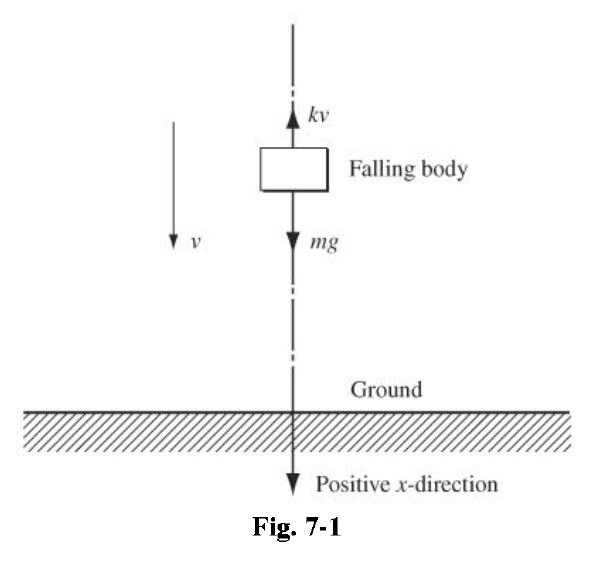
\includegraphics[height=7cm,keepaspectratio=true]{./edo/img020501.png}
		% img020501.png: 0x0 pixel, 300dpi, 0.00x0.00 cm, bb=
		\label{fig:020501}
	\end{figure}
	



	En nuestro modelo, $F= mg - kv,$ donde $m$ es la masa, $g$ es la aceleración debida a la gravedad y $k>0$ es una constante de proporcionalidad debida a la resistencia del aire.



	De manera que obtenemos la ecuación diferencial $mg-kv=m\dfrac{dv}{dt},$ o de manera equivalente
	\[
		\label{bron:7.4}
		\dfrac{dv}{dt}+\dfrac{k}{m}v=g.
	\]
	



% 
%  \begin{problema}
%   Una bola de acero que pesa 2 lbs se deja caer desde una altura de 3000 pies sin velocidad. Mientras cae, encuentra una resistencia del aire (numéricamente) igual a $\frac{v}{8}$ (en libras), donde $v$ indica la velocidad de la bola (en pies sobre segundo). Encuentre
%   \begin{enumerate}
%    \item la velocidad límite para la bola;
%    \item y el tiempo requerido para que bola impacte en el suelo.
%   \end{enumerate}
%
%  \end{problema}
%
% 

{}
	\begin{problema}
		Un cuerpo que pesa \texttt{64lbs} es dejado caer desde una altura de \texttt{100fts} con velocidad inicial de \texttt{10ft/sec.}
		
		Suponga que la resistencia del aire es proporcional a la velocidad del cuerpo. Se sabe que la velocidad límite del cuerpo es de \texttt{128ft/sec}. Encuentre:
		\begin{enumerate}
			\item una expresión para la velocidad del cuerpo en cualquier tiempo $t$,  y
			\item una expresión para la posición del cuerpo en cualquier tiempo.
			\item Determine el instante en que choca contra el suelo.
		\end{enumerate}
		
	\end{problema}
	


\subsection{Ejemplos de Disolución}


	Consideremos un tanque que inicialmente contiene $V_{0}$ litros de salmuera, que contiene $Q_{0}$ kgs de sal.\\
	
	Otra solución de salmuera, que contiene $b$ kgs por litro se vierte en el tanque a una tasa o ritmo de $e$ litros/minuto en tanto que simultáneamente, la solución bien agitada abandona el tanque a un ritmo de $f$ litros/minuto.\\
	
	El problema es encontrar la cantidad de sal en el tanque en respecto del tiempo $t.$



	\begin{figure}
		\centering
		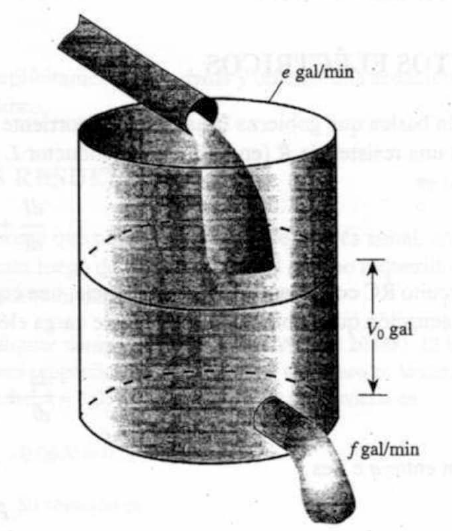
\includegraphics[height=5cm,keepaspectratio=true]{./edo/img020506.png}
		% img020506.png: 0x0 pixel, 300dpi, 0.00x0.00 cm, bb=
		\label{fig:020506}
	\end{figure}
	




	Por $Q$ denotaremos la cantidad (en kilos) de sal que se encuentra en el tanque en en el tiempo $t.$\\
	
	El volumen de salmuera al tiempo $t$ es
	\[
		\label{bron:7.7}
		V(t)=V_{0}+e\times t-f\times t.
	\]
	



	La concentración de sal en el tanque en un momento dado es $$\dfrac{Q(t)}{V(t)},$$ de lo que se deduce que la sal sale del tanque a una tasa de
	$$
	f \times \left( \dfrac{Q(t)}{V(t)} \right)
	\texttt{kgs/min.}
	$$



	De este modo,
	$$
	\dfrac{dQ}{dt}=be-f\times \left( \dfrac{Q}{V_{0}+(e-f)t} \right),
	$$
	o de manera equivalente
	\[
		\label{bron:7.8}
		\dfrac{dQ}{dt}+f \times \left( \dfrac{Q}{V_{0}+(e-f)\times t} \right)=be.
	\]
	



	\begin{problema}
		\label{bron:exmp:7.17}
		Un tanque contiene inicialmente $100$ litros de una solución de salmuera con $1$ kilo de sal. En $t=0$ se vierte otra solución de salmuera que contiene $1$ kilo de sal por litro a un ritmo de $3$ litros/minuto, en tanto que la salmuera bien agitada abandona el tanque al mismo ritmo. Encuentre
		\begin{enumerate}
			\item la cantidad de sal en el tanque en cualquier tiempo $t,$ y
			\item el tiempo en el cual la mezcla en el tanque contiene 2 kilos de sal.
		\end{enumerate}
		
	\end{problema}
	



	\begin{problema}
		Un tanque de 50 lts contiene inicialmente $10$ litros de agua fresca. Al tiempo $t=0$ se vierte al tanque una solución de salmuera que contiene $1$ kilo de sal por litro a un ritmo $4$ lts/min, mientras que la mezcla bien agitada abandona el tanque a un ritmo de $2$ lts/min. Encuentre
		\begin{enumerate}
			\item la cantidad de tiempo requerido para que ocurra un derrame y;
			\item la cantidad de sal en el tanque al momento del derrame.
		\end{enumerate}
		
	\end{problema}
	



\subsection{Circuitos Eléctricos}


	La ecuación básica que gobierna la cantidad de corriente $I$ (en amperios) en un circuito $RL$ simple (fig. \ref{fig:020502}) consiste en una resistencia $R$ (en ohmios), un inductor $L$ (en henrios) y una fuerza electromotriz (abreviado fem)$E$ (en voltios) es
	\[
		\label{bron:7.9}
		\dfrac{dI}{dt}+\dfrac{R}{L}I=\dfrac{E}{L}.
	\]
	



	\begin{figure}
		\centering
		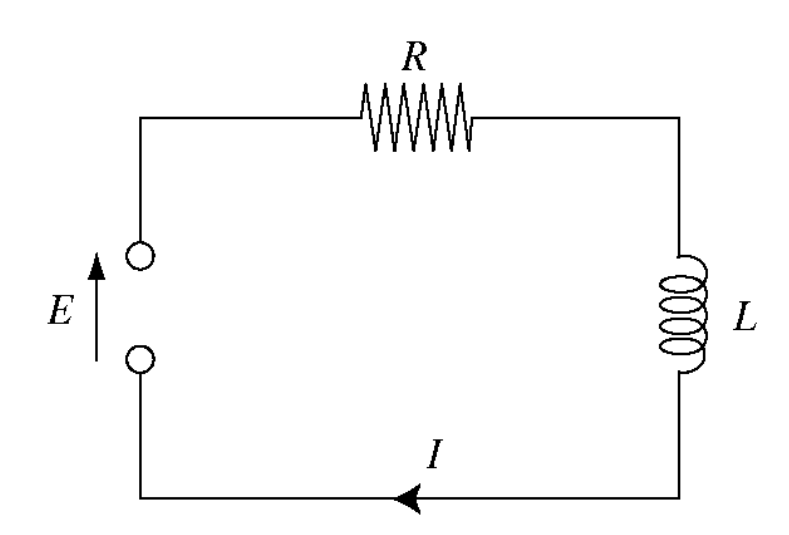
\includegraphics[height=5cm,keepaspectratio=true]{./edo/img020502.png}
		% img020502.png: 0x0 pixel, 300dpi, 0.00x0.00 cm, bb=
		\label{fig:020502}
	\end{figure}
	



	\begin{problema}
		Un circuito $RL$ tiene una $fem$ de 5 voltios, una resistencia de 50 ohmios, una inductancia de 1 henrio y no tiene corriente inicial. Encuentre la corriente de estado estacionario, i.e., cuando $t\to \infty.$
	\end{problema}
	



	\begin{figure}
		\centering
		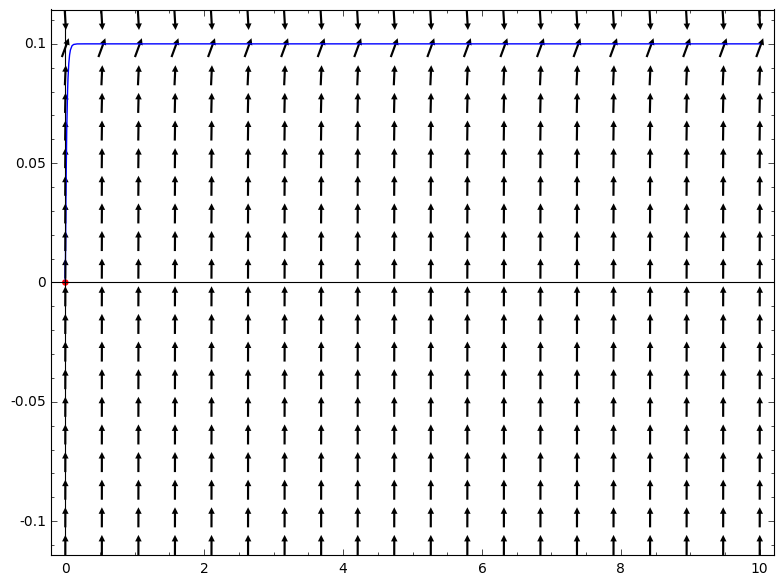
\includegraphics[height=5cm,keepaspectratio=true]{./edo/img020504.png}
		% img020504.png: 0x0 pixel, 300dpi, 0.00x0.00 cm, bb=
		\label{fig:020504}
	\end{figure}
	




	Para un circuito $RC$ consistente en una resistencia, una capacidad $C$ (en faradios), una fem y sin inductancia (fig. \ref{fig:020503}), la ecuación que gobierna la cantidad de carga eléctrica $q$ (en coulombios) sobre el capacitor es
	\[
		\label{bron:7.10}
		\dfrac{dq}{dt}+\frac{1}{R\cdot C}q=\dfrac{E}{R}.
	\]
	



	\begin{figure}
		\centering
		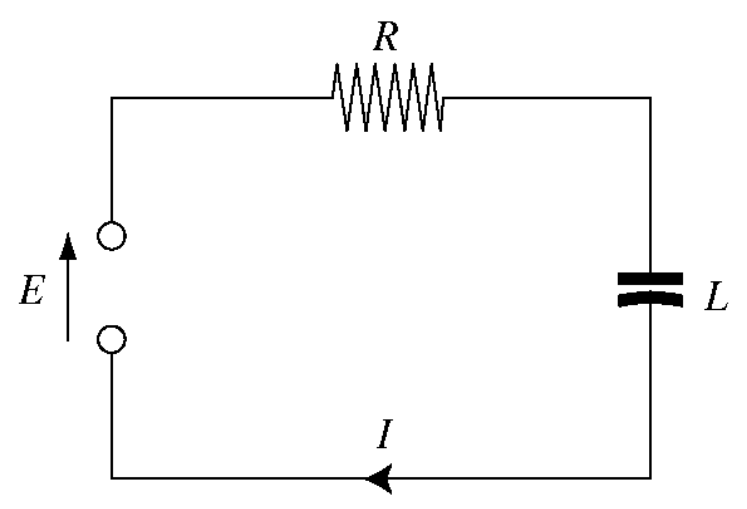
\includegraphics[height=5cm,keepaspectratio=true]{./edo/img020503.png}
		% img020502.png: 0x0 pixel, 300dpi, 0.00x0.00 cm, bb=
		\label{fig:020503}
	\end{figure}
	



	La relación entre $q$ e $I$ es
	\[
		\label{bron:7.11}
		I=\dfrac{dq}{dt}.
	\]
	



{}
	\begin{problema}
		Un circuito \texttt{RC} tiene una \texttt{fem} dada por $400\cos(2t),$ una resistencia de \texttt{100 ohms} y una capacitancia de \texttt{1/100 faradios}. No existe carga inicial en el capacitor. Encuentre la corriente del circuito en función del tiempo, y determine su comportamiento asintótico.
	\end{problema}
	




	\begin{problema}
		Un circuito $RL$ tiene una $fem$ (en voltios) dada por $3sin(2t),$ una resistencia de 10 ohmios, una inductancia de 0.5 henrios y una corriente inicial de 6 amperios.
		
		Encuentre la corriente de estado estacionario.
	\end{problema}
	


	\begin{figure}
		\centering
		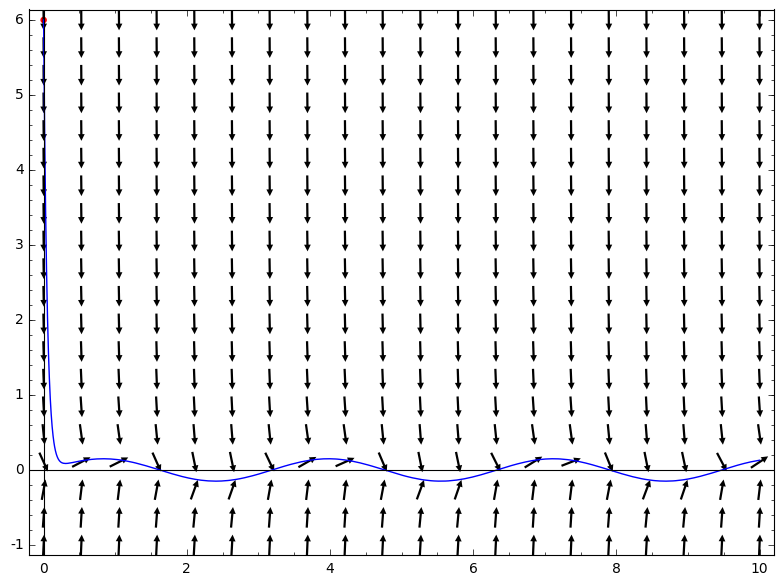
\includegraphics[height=5cm,keepaspectratio=true]{./edo/img020505.png}
		% img020504.png: 0x0 pixel, 300dpi, 0.00x0.00 cm, bb=
		\label{fig:020505}
	\end{figure}
	











